\section{Introduction}

%TL;DR of paragraph: interiors are why a generated building is useful, and no exterior view shows them.
Many of us are taught at a young age that we shouldn't judge a book by its cover. A building can be examined the same way. It may have rooms, doors--an interior. And, in many cases, structures rely on these interior layouts to make them usable rather than decorative. Consider a Minecraft build someone walks through, a LEGO model someone assembles, or an indoor environment that needs navigable space and collision volumes for robotic training.

%TL;DR of paragraph: the field generates discrete 3D structure well, inherited its evaluation protocol from image generation, and already lists the defect as a caveat.
Generative models of discrete {3D} structure have advanced quickly, over LEGO
assemblies \citep{pun2025brickgpt,legoace, kulits2026bricknet}, sparse voxel categories
\citep{jung2025scaffold}, Minecraft worlds \citep{merino2026dreamcubed} and
serialized geometry \citep{wang2024llamamesh,sudhakaran2023mariogpt}. Many of their evaluation techniques come from image generation where they render a structure from a handful of views, embed the renders with a pretrained encoder such as DINOv2 \citep{oquab2024dinov2}, and report a Fr\'echet inception distance (FID) \citep{heusel2017fid} or kernel inception distance (KID) \citep{binkowski2018kid} between the generated and real feature distributions. We call this family \emph{render-and-embed}. Its limitation is already on the record. The largest generative study in this domain \citep{merino2026dreamcubed} lists among its own limitations that render-based FID ``struggles to assess internal structure (e.g., whether a building has a coherent interior),'' then ranks models with it for want of an alternative. What the field lacks is a measurement of how large the effect is and a metric that sees what it misses. We supply both.

\begin{figure}[t]
\centering
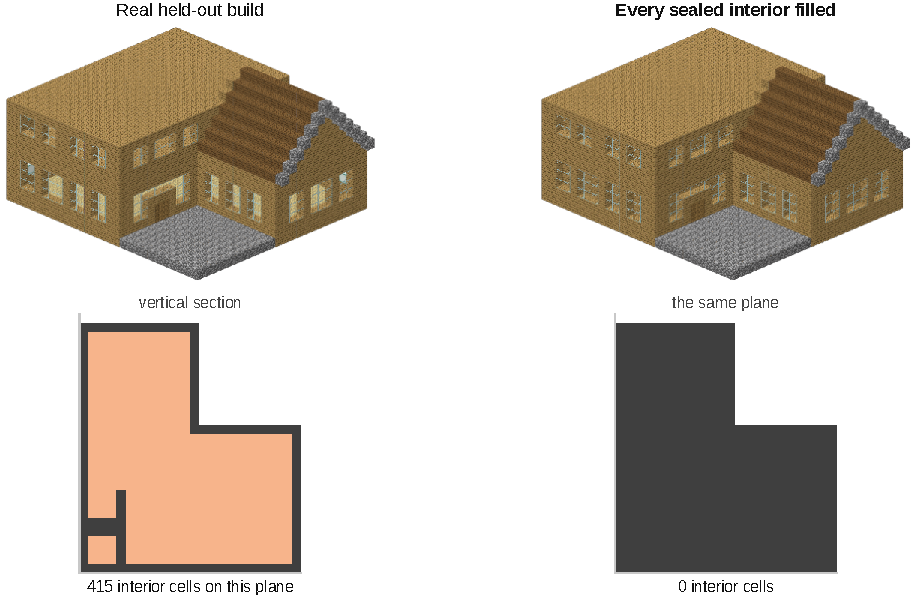
\includegraphics[width=\linewidth]{figures/fig1_teaser}
\caption{\textbf{A building is not its silhouette.} \emph{Left:} a real build, sectioned vertically through its five rooms, with sealed interior air in peach. \emph{Right:} the same build under \solidify{}, every sealed void filled by its own dominant material and cut on the same plane, almost indistinguishable in all four views the metric renders. Raw \mvkid{} moves from $-0.001$ to $+0.000$, one significance group, while \vkid{} moves $202$ noise floors. Renders use the metric's own texture pack; published builds
come from 3D-Craft (Appendix~\ref{app:data}).}
\label{fig:teaser}
\end{figure}

%TL;DR of paragraph: the probe is filling sealed interiors with the build's own material, and the render metric ties it with real data even though the metric is wide awake on the same corpus.
Our probe, \solidify{}, takes real buildings and fills every enclosed air cell with that build's own dominant material, so no new material betrays the corruption (Figure~\ref{fig:teaser}). It adds a median of $33\%$ more blocks, alters $94\%$ of examined builds, and leaves the exterior silhouette untouched. Scored at $n{=}128$ against $399$ held-out real builds, a solidified corpus and its genuine, real data counterpart \emph{share a significance group} under a paired, \com{What does this mean haha? These two last lines} Holm-corrected \citep{holm1979simple} comparison over all arm pairs. The same encoder and the same statistic separate a material permutation of the same builds at $+220.83$ noise floors (Table~\ref{tab:leaderboard}).

%TL;DR of paragraph: the cutaway ablation locates the failure in the view protocol rather than the encoder, and under an opaque renderer the invisibility is exact.
\com{weakish? Hard to follow--maybe too much bloat, see what really adds something in this paragraph}
The failure is in what the views show, not in what the encoder computes.
Holding the encoder and the statistic fixed and changing only the cameras, so
that the renders expose the interior, separates the same probe at $9$-$57$
noise floors (\S\ref{sec:ablation}). Under an opaque renderer the invisibility
is exact as filling sealed voids cannot change any
exterior view, so no encoder, statistic, sample size or view budget separates a
corpus from its solidified copy (\S\ref{sec:hollow},
Appendix~\ref{app:hull}).

%TL;DR of paragraph: the prescription is to validate a metric against corruptions of known severity before ranking with it, and to measure geometry directly alongside the renders.
\com{what does this line mean} A metric should therefore earn the right to rank. We score candidate metrics
against corruptions of known severity and require monotonicity, invariance and
sample-size stability before any of them orders a scoreboard, with separate
disqualification gates for memorization and mode collapse. Measuring geometry
directly, alongside the renders rather than instead of them, closes the blind
spot. We make three main contributions.

\begin{enumerate}[leftmargin=*,itemsep=1pt,topsep=2pt]

\item \textbf{Interior blindness, and it belongs to the representation}
(\S\ref{sec:blindness}--\ref{sec:hollow}). Render-and-embed distances cannot
distinguish a corpus of real buildings from the same corpus with every interior
filled, while the same test resolves every corruption that reaches the exterior.
Seven render-space statistics, five encoders, view budgets up to sixteen views
and a second domain all fail the same probe, and cutaway renders recover it with the same encoder
and the same statistic.

\item \textbf{A geometric metric with the complementary blindness}
(\S\ref{sec:method}). \vkid{} is a kernel distance on D4-invariant voxel
descriptors. It separates the probe by $202$ noise floors, needs no GPU, and is
\emph{exactly} invariant to material permutation, so neither metric alone ranks
both corruptions correctly.

\item \textbf{A validation protocol, and a suite that implements it}
(\S\ref{sec:method}). Gates on ordering, invariance and $n$-stability decide
whether a metric may rank anything at all. Fr\'echet distance, the functional form FID
uses, fails $n$-stability, as do coverage, recall and the biased maximum mean discrepancy
(MMD) estimator \citep{jayasumana2024cmmd}; precision and density
\citep{naeem2020prdc,kynkaanniemi2019precision} fail monotonicity.

\end{enumerate}
